\documentclass[journal, a4paper]{IEEEtran}
\usepackage[utf8]{inputenc}
\usepackage{cite}
\usepackage{graphicx}
\usepackage{url}
\usepackage{float}
\usepackage[flushleft]{threeparttable}
\usepackage{amsmath}

\renewcommand{\abstractname}{Resumo}
\renewcommand{\tablename}{TABELA}
\renewcommand{\refname}{Referências}

\begin{document}
	\title{Relatório de Implementação: \textit{Simulated Annealing} e Algoritmo Genético para solução do problema do Caixeiro Viajante}
	\author{Rodolpho Pivetta Sabino}
	\markboth{Universidade Estadual de Mato Grosso do Sul \newline Inteligência Artificial - Prof. Dr. Osvaldo Vargas Jacques}{}
	\maketitle

\begin{abstract}
	Na área da computação existem problemas que são tão grandes que tornam sua solução impossível computacionalmente. Exemplos desses tipos de problemas são problemas de otimização combinatória. Dentro dessa classificação, existe o Problema do Caixeiro Viajante. Este relatório busca apresentar resultados comparativos das implementações de algoritmos para solução desse problema. Os algoritmos \textit{Simulated Annealing} e Algoritmo Genético são boas ferramentas para soluciona-lo. Com isso, é possível observar as vantagens e desvantagens de se utilizar tais algoritmos.
\end{abstract}

\section{Introdução e Contextualização}
	\PARstart{O}{} Problema do Caixeiro Viajante (PCV) é conhecido pela sua complexidade. Em um contexto simples, existe um caixeiro viajante que deseja visitar um conjunto de cidades no menor percurso possível para que cada cidade seja visitada apenas uma única vez. Este problema tem inúmeras aplicações práticas, como por exemplo a implementação de sistemas digitais, minimização de rotas de veículos, sequenciamento de atividades, entre outros.

    Este problema, em termos computacionais, é um exemplo de problema de otimização combinatória. A formulação desse problema se dá por encontrar o número \texttt{R(n)} de rotas para o caso de \texttt{n} cidades, utilizando um raciocínio combinatório simples. Em um exemplo de \texttt{n = 4} cidades, a primeira e a última posição são fixas; a segunda posição pode assumir qualquer uma das 3 cidades restantes; a terceira posição pode assumir qualquer uma das 2 cidades restantes; e por fim a quarta posição assume a cidade restante \cite{portocv}. O número de rotas pode ser calculado como $3 * 2 * 1 = 6$.

    Desse modo, como a primeira posição é fixa, esse problema pode ser descrito utilizando a notação fatorial, o que resulta em:
    \begin{equation}
		R(n) = (n - 1)!
	\end{equation}

	A execução computacional desse problema em termos gerais e a fim de comparação, pode ser visualizada na Tabela~\ref{tab:execucao}.

    \begin{table}[!hbt]
		\begin{center}
		\caption{Execução do problema do caixeiro viajante}
		\label{tab:execucao}
		\begin{tabular}{|c|c|c|c|}
			\hline
            \textbf{n}  & \textbf{Rotas por Segundo} & \textbf{$(n-1)!$} & \textbf{Tempo} \\
			\hline
			5  & 250 milhões & $24$ & insignificante \\
			\hline
			10 & 110 milhões & $362880$ & 0.003 seg \\
			\hline
			15 & 71 milhões & 87 bilhões & 20 min \\
			\hline
			20 & 53 milhões & $1.2*10^{17}$ & 73 anos \\
			\hline
			25 & 42 milhões & $6.2*10^{23}$ & 470 milhões de anos \\
            \hline
		\end{tabular}
        \begin{tablenotes}
            Fonte: Adaptada de \cite{portocv}
        \end{tablenotes}
		\end{center}
	\end{table}

	Como pode ser visto, até mesmo para um número muito pequeno de cidades, o problema se torna extremamente grande, impossibilitando sua solução. Por essa razão o problema do caixeiro viajante é categorizado como NP-Completo, ou seja, faz parte de uma classe de problemas para os quais não existem algoritmos polinomiais em séries temporais determinísticos.

    Porém, para tal problema existem algoritmos de otimização combinatória capazes de encontrar boas soluções para grandes amostras. \textit{Annealing} consiste em um processo utilizado para fundir metais, onde estes são aquecidos a altas temperaturas e em seguida resfriados lentamente, transformando o produto final em uma massa homogênea. O \textit{Simulated Annealing} (SA) surgiu no contexto da mecânica estatística, desenvolvido por Kirkpatrick, Gelatt e Vecchi em 1983 e independentemente por Cerny em 1985, utilizando o algoritmo de Metrópolis de 1953 \cite{haeser}.

    Já o algoritmo genético (AG) é inspirado na maneira como o \textit{darwinismo} explica o processo de evolução das espécies, que consiste nas etapas de inicialização, avaliação, seleção, cruzamento, mutação, atualização e finalização. Basicamente, o AG cria uma população de possíveis respostas para o problema a ser tratado (inicialização) para depois submetê-la ao processo de evolução \cite{diogo}.

\section{Desenvolvimento}
	O processo de implementação dos algoritmos SA e AG se deram com base nos algoritmos implementados por \cite{lee}.

    Com relação à implementação, o algoritmo SA consiste em manter uma variável de temperatura e um fator de resfriamento, e a cada iteração, essa temperatura abaixa em relação ao fator de resfriamento. Aplicado ao PCV, o que define o resfriamento é o tamanho do percurso para um determinado conjunto de cidades, ou seja, a distância ao executar todo o percurso.

    Para que essa temperatura ser aceita, existem duas condições: (1) se a solução vizinha é melhor que a solução atual, essa solução é aceita de imediado; caso contrário (2) é preciso verificar quanto pior a solução é vizinho e como é a elevação da ``temperatura'' atual do sistema. Em altas temperaturas, o sistema é mais propício a aceitar soluções que são piores. Essa condição é definida pela seguinte formula:
    \begin{equation}
		e^{\frac{solutionEnergy - neighbourEnergy}{temperature}}
	\end{equation}
    Basicamente, quanto menor for a variação de energia (a qualidade da solução), e quanto maior a temperatura, é mais provável que o algoritmo aceite a solução.

    Já a implementação do AG consiste em seguir os seguintes passos:
    \begin{itemize}
    \item Inicialização - Cria uma população inicial gerada aleatoriamente de tamanho pré-definido.
	\item Avaliação - Cada membro da população é avaliado e então calculada uma ``aptidão'' para tal indivíduo. Esse valor é calculado com base em requisitos pré-definidos.
	\item Seleção - Seleciona os melhores indivíduos da população. Existem alguns métodos de seleção diferentes, mas a ideia básica é escolher os melhores indivíduos para gerar novas populações.
	\item \textit{Crossover} - Consiste em combinar indivíduos. Análoga a reprodução de espécies na natureza. O desejado é que através da combinação de certos traços de dois ou mais indivíduos, crie-se indivíduos que herdam as melhores características de cada um de seus pais.
	\item Mutação - Consiste em inserir aleatoriedade na geração de indivíduos, fazendo mudanças pequenas para um genoma de indivíduos.
	\end{itemize}

\section{Resultados}
	Foram realizados testes comparativos em relação à qualidade da solução encontrada para um mesmo conjunto inicial de cidades (com percursos iniciais diferentes, gerados aleatoriamente) do PCV sendo resolvido pelos algoritmos SA e AG. Os testes foram executados para amostras de 25, 50, 75 e 100 cidades.

    Para a execução dos algoritmos, foi utilizado um computador com as especificações descritas na Tabela~\ref{tab:especificacoes}.

    \begin{table}[!hbt]
		\begin{center}
		\caption{Especificações do computador de execução}
		\label{tab:especificacoes}
		\begin{tabular}{|l|l|}
			\hline
			Processador  & Intel\copyright Core i3-3110M CPU 2.40GHz x 2 \\
			\hline
			Memória RAM & 7.7GiB \\
			\hline
			Sistema Operacional & Linux Mint 17.1 64-bit \\
			\hline
			Kernel & 3.13.0-37-generic \\
			\hline
		\end{tabular}
        \begin{tablenotes}
            Fonte: Elaborada pelo autor
        \end{tablenotes}
		\end{center}
	\end{table}

    A implementação foi feita utilizando a linguagem Python, que é uma linguagem de programação de alto nível, interpretada, orientada a objetos e de tipagem dinâmica e forte criada por Guido van Rossum em 1990 \cite{borges}. Foi utilizada também a biblioteca de plotagem 2D matplotlib.

    No algoritmo SA foi utilizada como temperatura inicial o valor de 1000 e o fator de resfriamento 0,0003. Para o AG foi utilizado 0,015 como fator de mutação e um tamanho de 5 cidades para torneio, com a geração de 1000 novas populações.

    Para o primeiro conjunto de cidades (25), o SA obteve melhor resultado, partindo de um percurso de distância 2606.1074, chegar ao resultado de 780.1820 enquanto o AG obteve 799.1782 para um conjunto inicial de distância 2594.8336. O comparativo pode ser visto na Fig.~\ref{fig:comp-25}.

    \begin{figure}[H]
		\begin{center}
		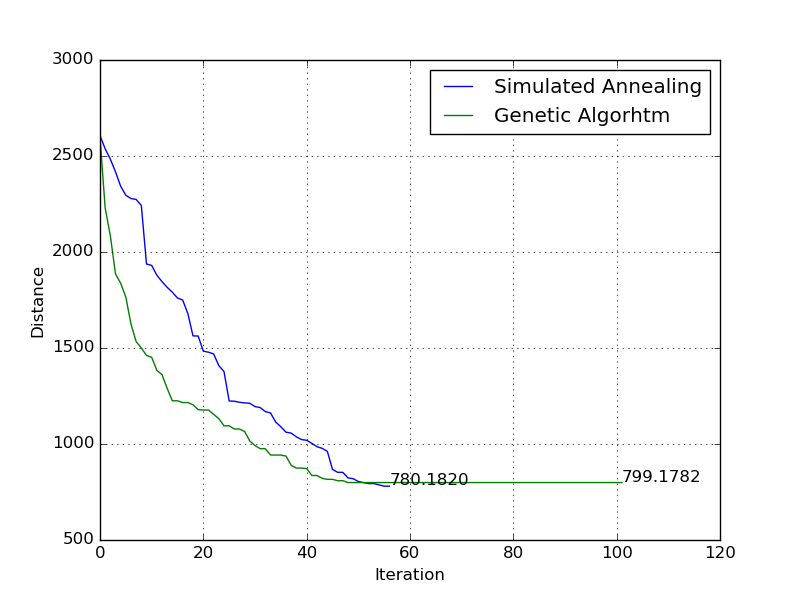
\includegraphics[width=\columnwidth]{25-comparacao.png}
		\caption{Convergência para a melhor solução: 25 cidades}
		\label{fig:comp-25}
		\end{center}
	\end{figure}

    Para o segundo conjunto de cidades (50), o AG obteve melhor resultado, com distância final igual a 1390.6086 no percurso inicial de distância 4903.8204, enquanto o SA obteve 1532.3218 para um conjunto inicial de distância 4897.6301. Esse comparativo é visto na Fig.~\ref{fig:comp-50}.

    \begin{figure}[H]
		\begin{center}
		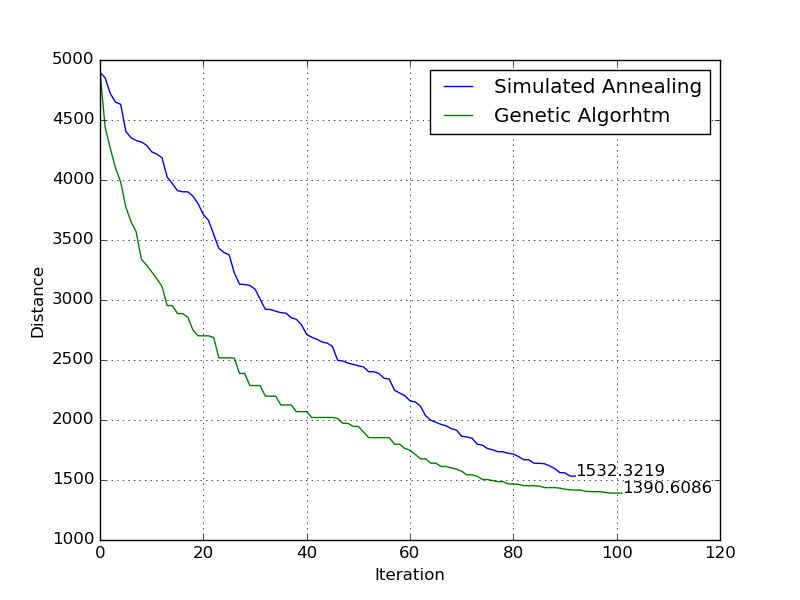
\includegraphics[width=\columnwidth]{50-comparacao.png}
		\caption{Convergência para a melhor solução: 50 cidades}
		\label{fig:comp-50}
		\end{center}
	\end{figure}

    Para o terceiro conjunto de cidades (75), novamente o SA obteve melhor resultado. Para o percurso inicial de distância 8157.4577, sua solução foi 2200.3268, enquanto para o percurso inicial de distância 8059.4831, o resultado final do AG foi 2919.2844 como pode ser visto na Fig.~\ref{fig:comp-75}.

    \begin{figure}[H]
		\begin{center}
		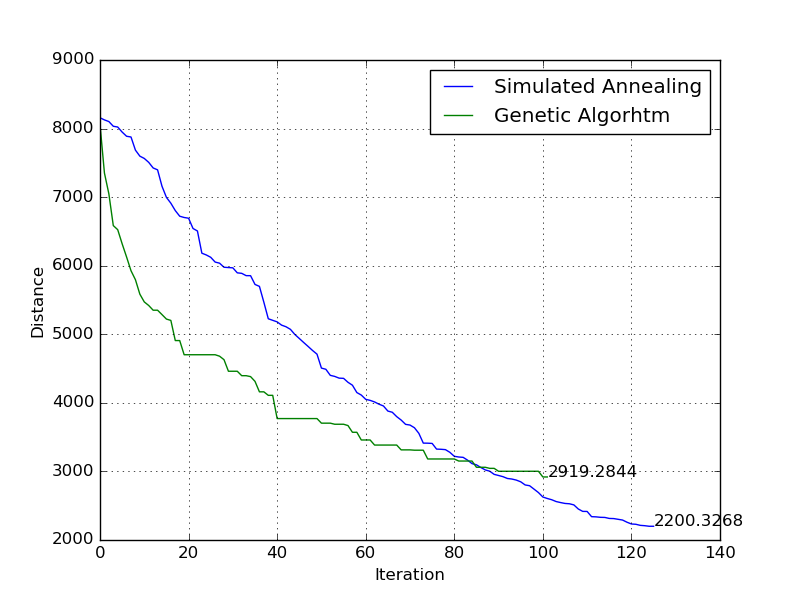
\includegraphics[width=\columnwidth]{75-comparacao.png}
		\caption{Convergência para a melhor solução: 75 cidades}
		\label{fig:comp-75}
		\end{center}
	\end{figure}

    Por fim, para o último conjunto de cidades (100), o resultado obtido pelo algoritmo SA foi novamente melhor que o AG. Para um conjunto inicial de distância 10631.0364, o SA obteve 3161.6052 de distância final, enquanto o AG com distância inicial de 11159.9226 obteve 4905.9245 de distância final, como pode ser visto na Fig.~\ref{fig:comp-100}.

    \begin{figure}[H]
		\begin{center}
		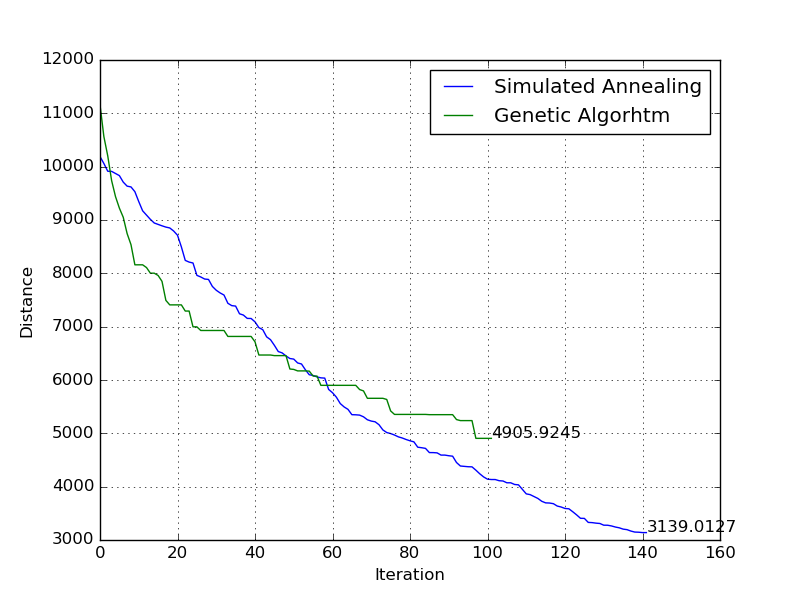
\includegraphics[width=\columnwidth]{100-comparacao.png}
		\caption{Convergência para a melhor solução: 100 cidades}
		\label{fig:comp-100}
		\end{center}
	\end{figure}

    É interessante observar nesse ponto que mesmo com uma grande diferença no resultado final, nenhuma das duas soluções são visivelmente satisfatórias. Observando as Figuras \ref{fig:100-simulated} e \ref{fig:100-genetic}, o percurso final das duas soluções não formam uma envoltória nas cidades, o que possivelmente seria a melhor solução.

    \begin{figure}[H]
		\begin{center}
		\fbox{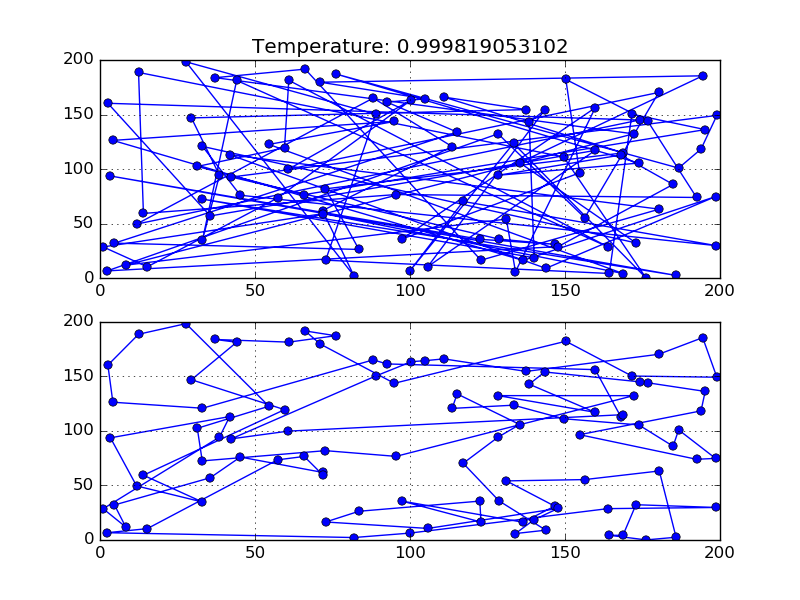
\includegraphics[width=\columnwidth]{100-simulated.png}}
		\caption{Solução final do SA}
		\label{fig:100-simulated}
		\end{center}
	\end{figure}

    \begin{figure}[H]
		\begin{center}
		\fbox{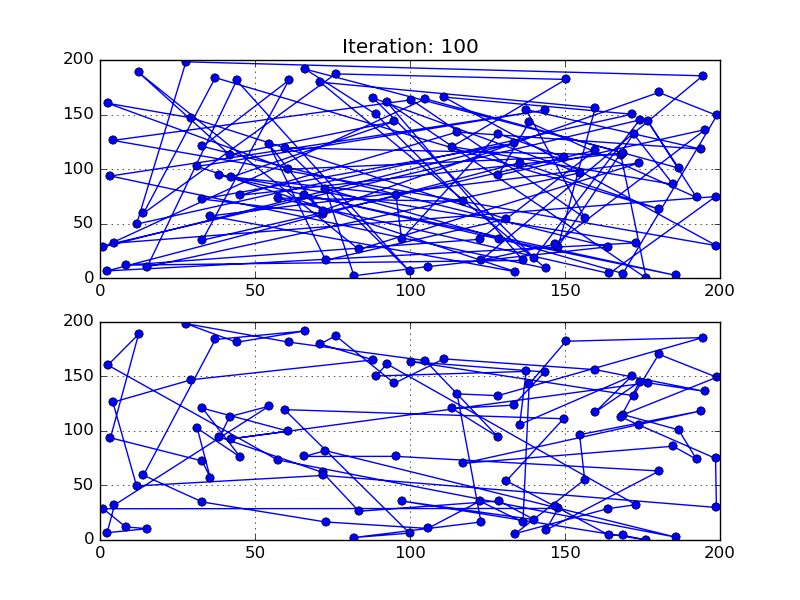
\includegraphics[width=\columnwidth]{100-genetic.png}}
		\caption{Solução final do AG}
		\label{fig:100-genetic}
		\end{center}
	\end{figure}


\section{Conclusão}
	Os resultados mostram que os algoritmos são bastante eficientes em encontrar boas soluções para o PCV, um problema complexo e extremamente grande. É possível notar que o SA tem uma grande vantagem em encontrar melhores resultados que o AG. Cabe aqui citar que o tempo de execução do AG é relativamente maior que o tempo de execução do SA, mesmo este fator não estar sendo avaliado neste trabalho, isso é um grande diferencial.

\begin{thebibliography}{5}
	\bibitem{diogo}
	C.~L.~Diogo. Algoritmos Genéticos: uma Introdução. 2002.
    \url{http://www.inf.ufrgs.br/~alvares/INF01048IA/ApostilaAlgoritmosGeneticos.pdf}

	\bibitem{haeser}
	G.~HAESER, M.~GOMES–RUGGIERO3. Aspectos Teóricos de Simulated Annealing e um Algoritmo duas Fases em Otimização Global. 2008.
	\url{https://www.ime.usp.br/~ghaeser/Hae_Gom.pdf}

    \bibitem{lee}
    J.~Lee. The Project Spot. 2015. \url{http://www.theprojectspot.com}.

	\bibitem{portocv}
	J.~F.~Porto da Silveira. Problema do Caixeiro viajante. 2002.
    \url{http://www.mat.ufrgs.br/~portosil/caixeiro.html}.

    \bibitem{borges}
    L.~E.~Borges. Python para Desenvolvedores. 2014.
\end{thebibliography}
\end{document}
